\documentclass[11pt,a4paper]{article}

\usepackage[utf8]{inputenc}
\usepackage[T1]{fontenc}
\usepackage[french]{babel}
\usepackage{lmodern}
\usepackage{microtype}
\usepackage[a4paper,margin=22mm,headheight=15pt,footskip=12mm]{geometry}
\usepackage{xcolor}
\usepackage{graphicx}
\usepackage{booktabs}
\usepackage{tabularx}
\usepackage{array}
\usepackage{amsmath}
\usepackage{enumitem}
\usepackage{titlesec}
\usepackage{fancyhdr}
\usepackage{hyperref}
\usepackage{caption}
\usepackage{float}

\definecolor{Navy}{HTML}{18324B}
\definecolor{MatrixBlue}{HTML}{3C7686}
\definecolor{ParallelPurple}{HTML}{6E45A3}
\definecolor{DetailBlue}{HTML}{154C75}
\definecolor{SelectOrange}{HTML}{E98E2E}
\definecolor{SelectDark}{HTML}{AB6821}
\definecolor{PaleBlue}{HTML}{EAF3F6}
\definecolor{PalePurple}{HTML}{F1EDF7}
\definecolor{PaleOrange}{HTML}{FBF1E4}
\definecolor{BodyText}{HTML}{334155}
\definecolor{SoftGray}{HTML}{64748B}
\definecolor{RuleGray}{HTML}{D9E2EA}

\hypersetup{
  colorlinks=true,
  linkcolor=Navy,
  urlcolor=MatrixBlue,
  citecolor=DetailBlue,
  pdftitle={Exploration visuelle du jeu de données Wine},
  pdfauthor={Ilyass Aftyss et Mohamed Reda Chawki}
}
\setlength{\parindent}{0pt}
\setlength{\parskip}{5pt}
\setlist[itemize]{leftmargin=1.4em,itemsep=2pt,topsep=3pt}
\setlist[enumerate]{leftmargin=1.7em,itemsep=3pt,topsep=3pt}
\titleformat{\section}{\Large\bfseries\sffamily\color{Navy}}{\thesection}{.65em}{}[\color{RuleGray}\titlerule]
\titleformat{\subsection}{\large\bfseries\sffamily\color{MatrixBlue}}{\thesubsection}{.65em}{}
\captionsetup{font=small,labelfont={bf,color=Navy},textfont={color=BodyText},skip=6pt}
\pagestyle{fancy}
\fancyhf{}
\fancyhead[L]{\small\sffamily\color{SoftGray}TP de visualisation · Wine}
\fancyhead[R]{\small\sffamily\color{SoftGray}D3.js · exploration multivariée}
\fancyfoot[C]{\small\sffamily\color{SoftGray}\thepage}
\renewcommand{\headrulewidth}{0.4pt}
\renewcommand{\headrule}{\hbox to\headwidth{\color{RuleGray}\leaders\hrule height \headrulewidth\hfill}}

\newcommand{\metric}[2]{\textcolor{#1}{\textbf{#2}}}
\newcommand{\smalltag}[1]{\begingroup\setlength{\fboxsep}{4pt}\colorbox{PaleBlue}{\sffamily\small\textcolor{Navy}{#1}}\endgroup}

\begin{document}

% Page de titre
\begin{titlepage}
\thispagestyle{empty}
\vspace*{11mm}
{\sffamily\bfseries\small\color{MatrixBlue} TRAVAUX PRATIQUES \hfill VISUALISATION EXPLORATOIRE}
\par\vspace{7mm}\noindent\color{MatrixBlue}\rule{\textwidth}{1.4pt}
\vspace{17mm}

{\sffamily\bfseries\color{ParallelPurple}\large RAPPORT DE TP}\par
\vspace{4mm}
{\sffamily\bfseries\color{Navy}\fontsize{34}{40}\selectfont Explorer les données Wine}\par
\vspace{5mm}
{\large\color{SoftGray}Matrice de dispersion, coordonnées parallèles et estimation de densité avec D3.js}\par
\vspace{13mm}

\begin{minipage}{.96\textwidth}
\setlength{\fboxsep}{13pt}
\colorbox{PaleBlue}{\parbox{\dimexpr\textwidth-2\fboxsep\relax}{
\sffamily\small\textcolor{Navy}{\textbf{Objectif}}\par
\vspace{2mm}
\normalfont\color{BodyText}Construire une page HTML/SVG interactive et utilisable hors ligne pour explorer les relations entre les mesures chimiques de 178 vins, sélectionner des observations de manière synchronisée et étudier la distribution d'une variable.
}}
\end{minipage}

\vspace{17mm}
{\sffamily\bfseries\color{Navy}\large Réalisé par}\par
\vspace{4mm}
\begin{tabularx}{.86\textwidth}{@{}X X@{}}
\smalltag{ÉTUDIANT·E 1} & \smalltag{ÉTUDIANT·E 2} \\
\textbf{Ilyass Aftyss} & \textbf{Mohamed Reda Chawki}
\end{tabularx}

\vfill
\noindent\color{RuleGray}\rule{\textwidth}{0.6pt}\par
\vspace{3mm}
\begin{tabularx}{\textwidth}{@{}X r@{}}
\small\sffamily\color{SoftGray}Jeu étudié : Wine recognition data · 13 variables numériques & \small\sffamily\color{SoftGray}\today
\end{tabularx}
\end{titlepage}

\tableofcontents
\thispagestyle{fancy}
\clearpage

\section{Résumé}
Ce travail met en œuvre les trois vues prescrites par le TP : une matrice de dispersion, des coordonnées parallèles et un histogramme superposé à une estimation de densité à noyau gaussien. L'application est développée en HTML, SVG et JavaScript avec D3.js v7.1.1. La bibliothèque et les données sont fournies localement : la page s'ouvre dans Chrome ou Chromium sans serveur ni connexion réseau.

Le fichier contient \metric{MatrixBlue}{178 observations} et \metric{MatrixBlue}{13 mesures numériques continues}. La colonne catégorielle de classe a été écartée afin de respecter la consigne de ne visualiser que les mesures numériques. Les brossages de la matrice et des axes parallèles pilotent une sélection commune, répercutée dans les trois vues.

\begin{quote}\small\color{Navy}\textbf{Résultat exploratoire principal.} La relation linéaire positive la plus marquée parmi les paires numériques est celle des phénols totaux et des flavanoïdes (corrélation de Pearson $r=0{,}865$). Cette association décrit les mesures observées ; elle ne constitue pas une relation causale.\end{quote}

\section{Contexte et objectifs}
Le TP demande une application interactive d'exploration multivariée réunissant, sur une même page, deux visualisations globales et une visualisation détaillée. Il demande également une sélection synchronisée, le choix de la dimension détaillée, ainsi que deux curseurs pour régler les classes de l'histogramme et le lissage gaussien~\cite{tp}.

Les objectifs de réalisation sont les suivants :
\begin{enumerate}
  \item comparer les variables deux à deux et rendre les associations visibles ;
  \item représenter simultanément le profil multivarié de chaque observation ;
  \item examiner la distribution d'une variable et modifier interactivement l'histogramme et la densité ;
  \item conserver les valeurs numériques d'origine et rendre la page autonome, sans serveur.
\end{enumerate}

\section{Données et préparation}
\subsection{Description du jeu}
Le fichier \texttt{wine.data} fourni contient 178 lignes et 14 champs : un identifiant de classe (1, 2 ou 3), puis 13 attributs numériques continus. Le fichier descriptif \texttt{wine.names} donne les noms des attributs et indique l'absence de valeurs manquantes~\cite{wine}. La colonne de classe n'est pas incluse dans les fichiers de visualisation : aucun identifiant de classe, regroupement ou code couleur de classe n'est utilisé.

La conversion conserve l'ordre des lignes et les valeurs des 13 variables. Aucun filtrage, remplacement de valeur ou centrage-réduction n'a été appliqué. Les fichiers livrés sont \texttt{wine.csv} et \texttt{wine.json}; \texttt{wine-data.js} expose le même tableau JSON par une variable JavaScript afin de permettre le chargement local avec l'URL \texttt{file://}, sans appel à \texttt{fetch()}.

\begin{table}[H]
\centering
\small
\caption{Étendue et moyenne des 13 mesures numériques (calculées sur les 178 observations).}
\label{tab:descriptives}
\begin{tabularx}{\textwidth}{@{}>{\raggedright\arraybackslash}Xrrr@{}}
\toprule
\textbf{Variable} & \textbf{Minimum} & \textbf{Maximum} & \textbf{Moyenne} \\
\midrule
Alcool & 11,03 & 14,83 & 13,001 \\
Acide malique & 0,74 & 5,80 & 2,336 \\
Cendres & 1,36 & 3,23 & 2,367 \\
Alcalinité des cendres & 10,60 & 30,00 & 19,495 \\
Magnésium & 70 & 162 & 99,742 \\
Phénols totaux & 0,98 & 3,88 & 2,295 \\
Flavanoïdes & 0,34 & 5,08 & 2,029 \\
Phénols non flavonoïdes & 0,13 & 0,66 & 0,362 \\
Proanthocyanidines & 0,41 & 3,58 & 1,591 \\
Intensité de couleur & 1,28 & 13,00 & 5,058 \\
Teinte & 0,48 & 1,71 & 0,957 \\
OD280/OD315 des vins dilués & 1,27 & 4,00 & 2,612 \\
Proline & 278 & 1680 & 746,893 \\
\bottomrule
\end{tabularx}
\end{table}

Les amplitudes et unités diffèrent fortement, en particulier pour la proline et le magnésium. Les vues multivariées utilisent donc une échelle propre à chaque variable pour exploiter l'espace graphique ; les histogrammes restent exprimés dans l'unité d'origine de la variable choisie.

\subsection{Écart explicite au critère de taille du TP}
Le document du TP recommande de choisir un jeu comportant au moins une quinzaine d'attributs. Le jeu Wine fourni ne possède que 13 mesures numériques, ou 14 champs en comptant la classe. La classe ayant été retirée conformément à la demande, l'application explore 13 dimensions : elle réalise les vues demandées, mais n'atteint pas le seuil de 15 attributs recommandé dans le sujet. Ce choix est conservé pour répondre à la consigne de travailler sur Wine et sur les seules données numériques.

\section{Conception des visualisations}
\subsection{Matrice de dispersion}
La matrice comporte 13 lignes et 13 colonnes : 156 cases hors diagonale pour les paires ordonnées et 13 petites distributions sur la diagonale. Chaque case hors diagonale encode une variable en abscisse et une autre en ordonnée. Un glisser-déposer dans une case sélectionne les observations contenues dans la zone. Les libellés de colonnes sont abrégés pour éviter leur chevauchement ; un survol révèle le nom complet et un clic choisit cette variable pour la vue détaillée.

\begin{figure}[H]
\centering
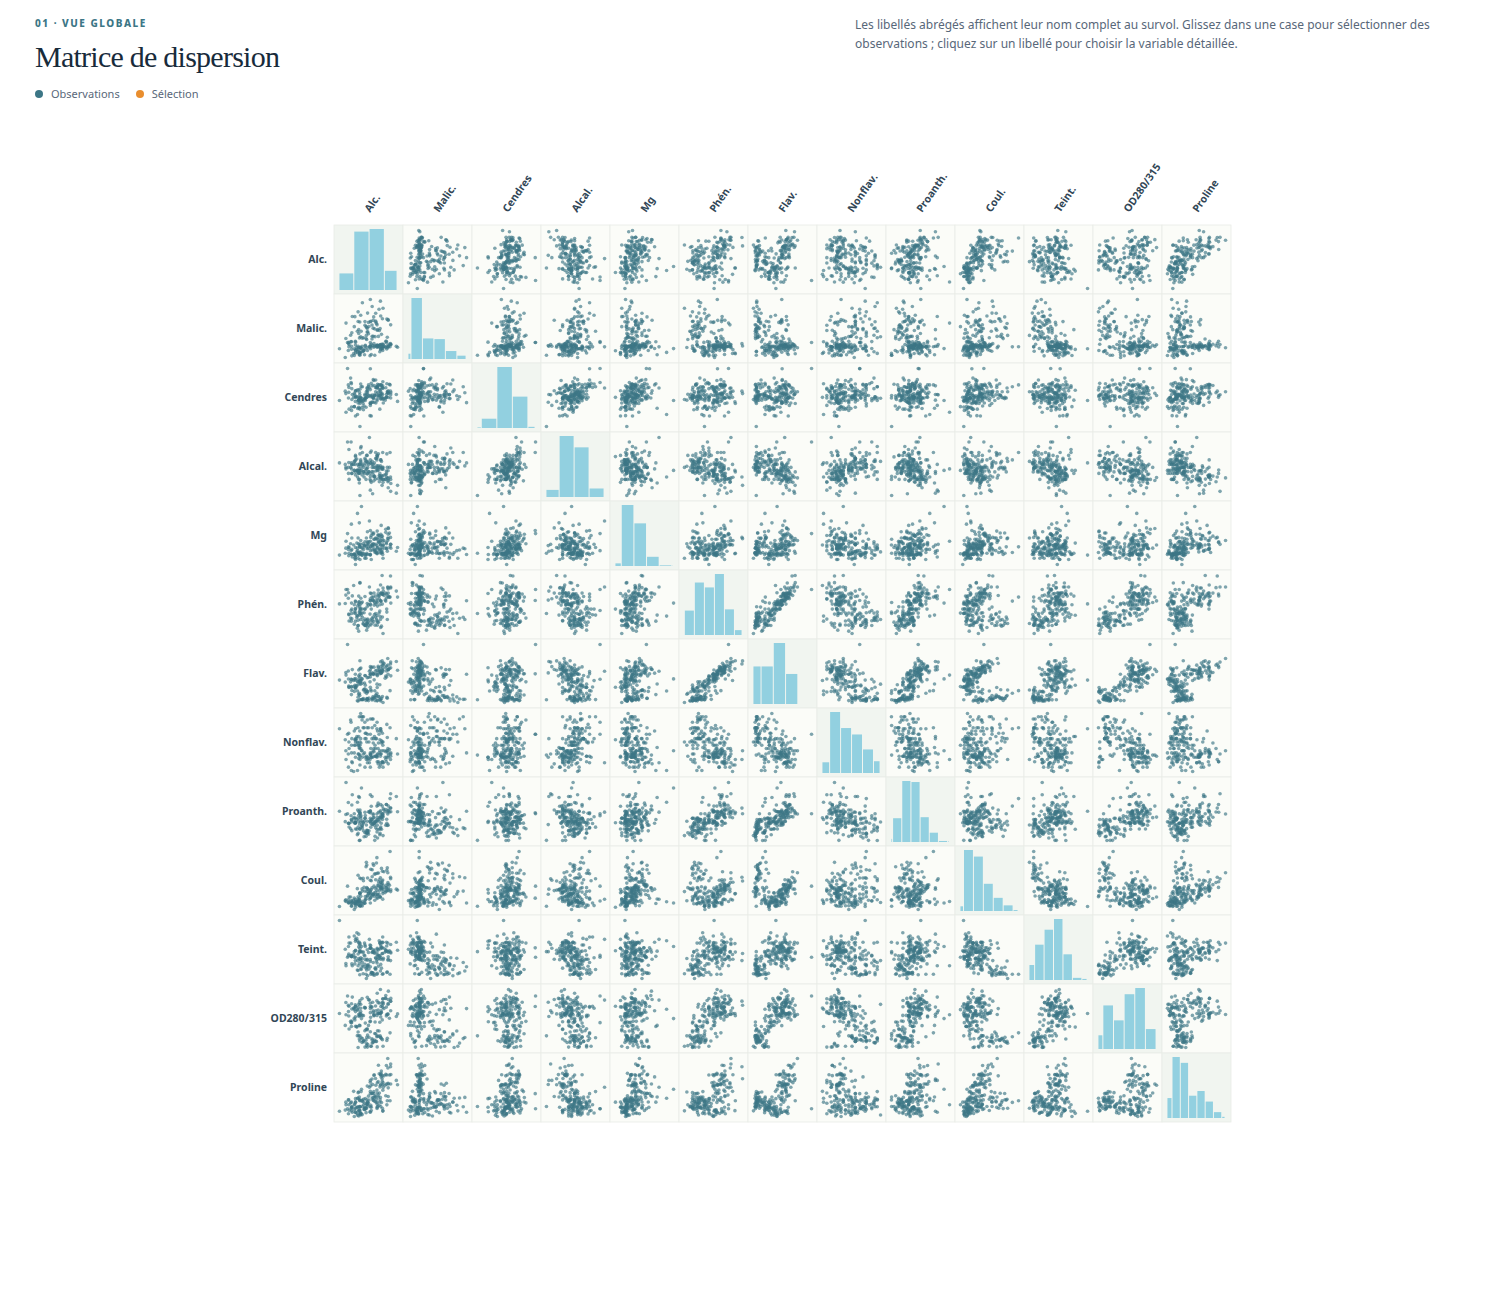
\includegraphics[width=.96\textwidth]{figures/matrice.png}
\caption{Matrice des 13 variables. Les cellules diagonales montrent les distributions marginales ; chaque cellule non diagonale compare une paire de mesures.}
\label{fig:matrice}
\end{figure}

\subsection{Coordonnées parallèles}
Chaque observation est tracée sous la forme d'une ligne qui relie ses valeurs sur les 13 axes. L'échelle verticale est calculée séparément pour chaque variable. Un brossage vertical sélectionne une plage sur un axe ; les sélections sur plusieurs axes sont combinées par intersection. Les noms courts restent horizontaux et le nom complet apparaît au survol.

\begin{figure}[H]
\centering
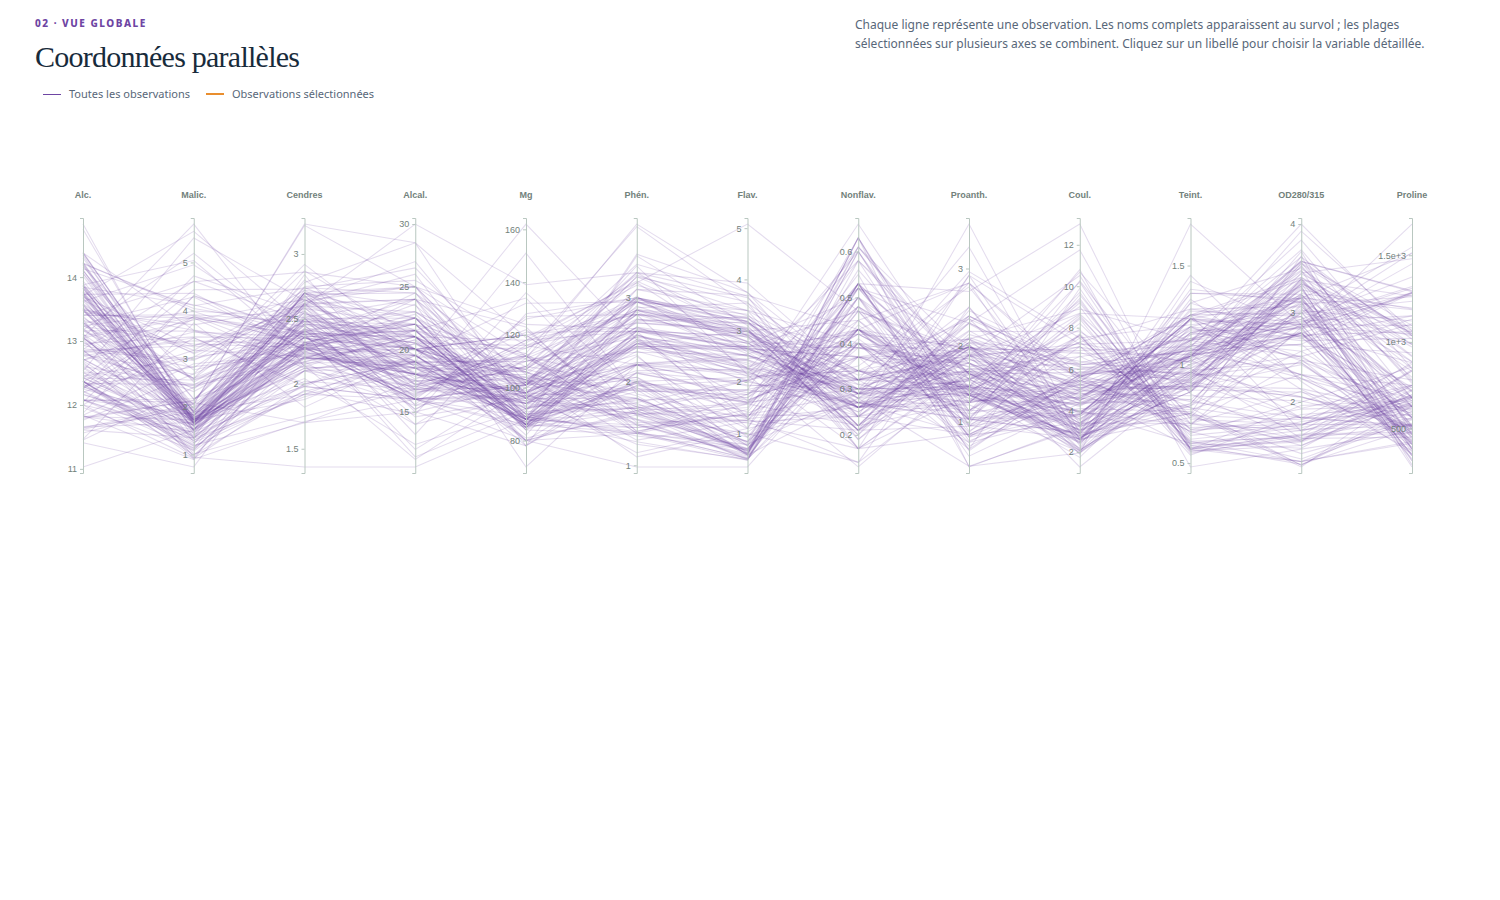
\includegraphics[width=.96\textwidth]{figures/coordonnees.png}
\caption{Coordonnées parallèles. Chaque polyline représente une observation ; les axes conservent les plages numériques propres aux attributs.}
\label{fig:paralleles}
\end{figure}

\subsection{Histogramme et densité gaussienne}
Un menu sélectionne la dimension à détailler ; le clic sur un libellé de la matrice ou des coordonnées parallèles met aussi à jour cette dimension. Le curseur « largeur des classes » ajuste la largeur des intervalles de l'histogramme. Le second curseur ajuste la largeur de bande $h$ de l'estimateur gaussien. Les plages des curseurs sont recalculées selon l'étendue de la variable.

Pour les observations $x_1,\ldots,x_n$, l'estimateur de densité est :
\[
  \widehat f_h(x)=\frac{1}{nh}\sum_{i=1}^{n}
  \varphi\!\left(\frac{x-x_i}{h}\right),
\]
où $\varphi$ est la densité de la loi normale centrée réduite. Comme l'histogramme est exprimé en effectifs, la courbe est multipliée par $n\,\Delta b$, où $\Delta b$ est la largeur de classe. Les deux représentations peuvent ainsi partager un même axe vertical sans présenter des unités incompatibles comme si elles étaient identiques.

\begin{figure}[H]
\centering
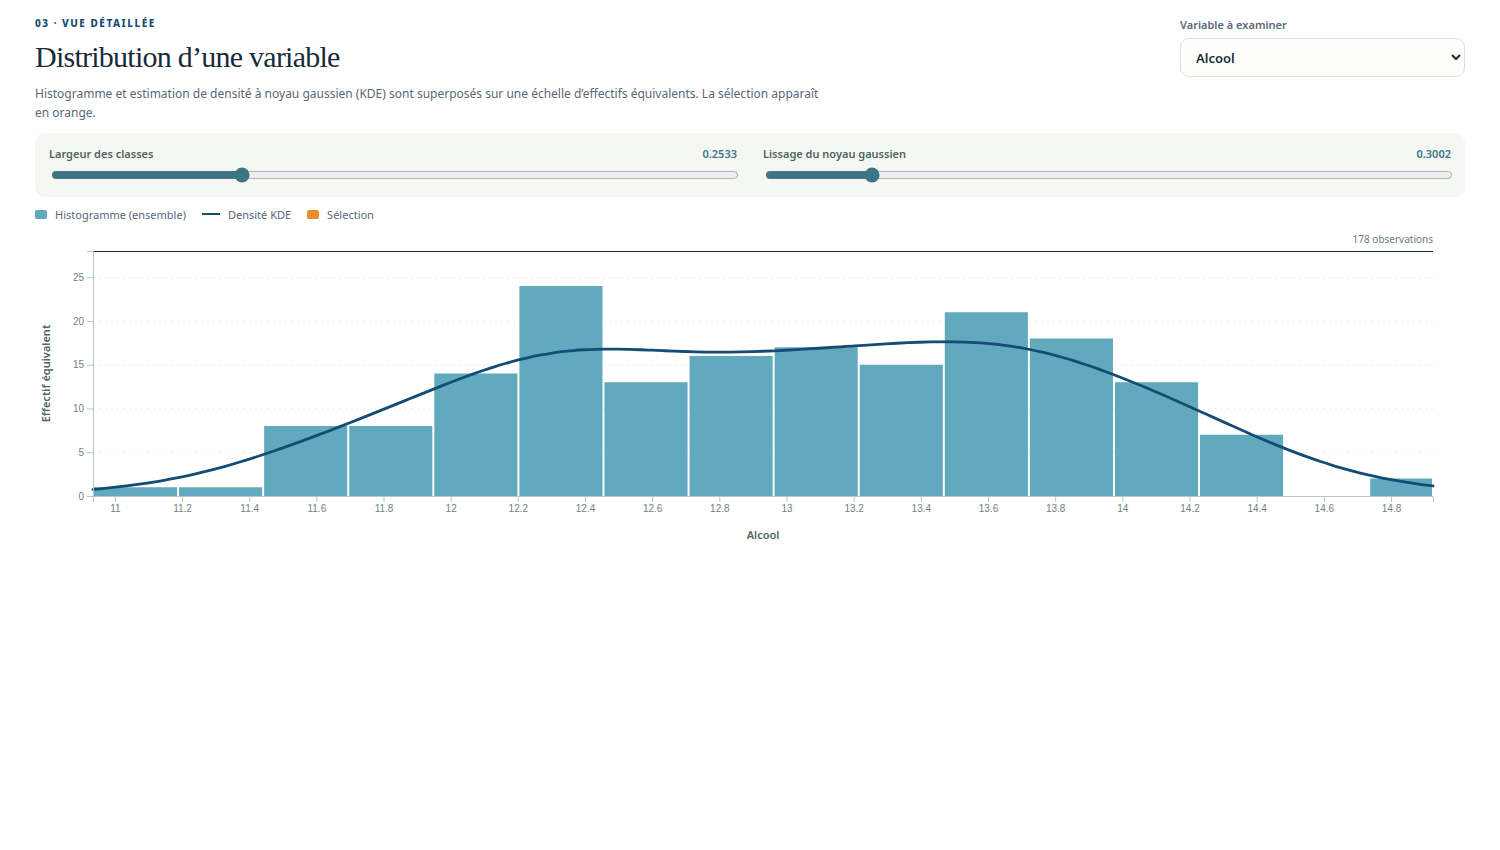
\includegraphics[width=.96\textwidth]{figures/distribution.png}
\caption{Distribution de l'alcool à l'état initial : histogramme et estimation KDE sur une échelle d'effectifs équivalents.}
\label{fig:distribution}
\end{figure}

\section{Réalisation et interactions}
\subsection{Organisation technique}
La page \texttt{index.html} charge uniquement des fichiers voisins : la feuille de styles, le code applicatif, les données JavaScript et D3.js v7.1.1 repris de l'archive d'exemple. Aucune police, feuille de style, donnée ou bibliothèque n'est récupérée en ligne. Les visualisations sont dessinées en SVG avec D3.js.

\subsection{Coordination des sélections}
La sélection est identifiée par un ensemble d'indices de lignes internes, sans ajouter de variable à \texttt{wine.json}. Lorsqu'une zone est brossée dans la matrice, les observations qui satisfont les deux intervalles choisis sont mises en évidence. Dans les coordonnées parallèles, chaque plage active ajoute une condition ; seules les observations satisfaisant toutes les plages restent sélectionnées. La couleur de sélection est reportée dans les autres cases de la matrice, les lignes parallèles, les barres et la courbe KDE de la distribution détaillée. Le bouton de réinitialisation efface les plages et rétablit l'affichage complet.

\subsection{Choix des couleurs et des libellés}
Chaque vue possède une couleur de base distincte : bleu pétrole pour la matrice, violet pour les coordonnées parallèles, cyan pour l'histogramme et bleu foncé pour la courbe KDE. L'orange indique la sélection. Les noms complets sont conservés dans les infobulles pour concilier lisibilité et identification précise des variables.

\section{Résultats et interprétation}
La corrélation de Pearson a été calculée sur les 13 colonnes numériques, sans utiliser la classe. Les paires ci-dessous sont des associations linéaires descriptives ; elles servent à confronter l'inspection de la matrice, et ne démontrent pas de causalité.

\begin{table}[H]
\centering
\small
\caption{Quelques corrélations observées entre variables numériques.}
\label{tab:correlations}
\begin{tabularx}{.92\textwidth}{@{}>{\raggedright\arraybackslash}X>{\raggedright\arraybackslash}Xr@{}}
\toprule
\textbf{Variable 1} & \textbf{Variable 2} & \textbf{$r$ de Pearson} \\
\midrule
Phénols totaux & Flavanoïdes & $+0{,}865$ \\
Flavanoïdes & OD280/OD315 des vins dilués & $+0{,}787$ \\
Phénols totaux & OD280/OD315 des vins dilués & $+0{,}700$ \\
Alcool & Proline & $+0{,}644$ \\
Acide malique & Teinte & $-0{,}561$ \\
Flavanoïdes & Phénols non flavonoïdes & $-0{,}538$ \\
Intensité de couleur & Teinte & $-0{,}522$ \\
\bottomrule
\end{tabularx}
\end{table}

Les associations positives entre phénols totaux, flavanoïdes et absorbance OD280/OD315 sont visibles sous forme de tendances croissantes dans la matrice. Des associations négatives apparaissent entre l'acide malique et la teinte, ainsi qu'entre les flavanoïdes et les phénols non flavonoïdes. Le graphe de densité permet par ailleurs d'examiner une distribution seule, mais le choix de $h$ modifie le niveau de détail : une bande étroite accentue les variations locales, une bande large les lisse.

Dans les coordonnées parallèles, la superposition de 178 lignes révèle les profils et les croisements, mais la forte densité peut masquer certaines observations. La sélection interactive est donc importante pour isoler une plage de profils. La classe étant exclue, aucune couleur ne permet d'attribuer visuellement les lignes aux trois catégories originales.

\section{Vérifications, limites et améliorations possibles}
\subsection{Vérifications effectuées}
\begin{itemize}
  \item concordance des 178 lignes entre le fichier source, le CSV numérique, le JSON et son enveloppe JavaScript ;
  \item vérification de 13 propriétés numériques par observation, sans colonne de classe ;
  \item ouverture locale dans Chromium et présence des trois SVG ;
  \item essais des curseurs, du menu de variable, du clic sur un libellé, des deux brossages, de la mise en évidence synchronisée et de la réinitialisation ;
  \item contrôle d'intégrité de l'archive de livraison.
\end{itemize}

\subsection{Limites}
Les variables sont de nature et d'échelle différentes ; chaque axe des vues globales est mis à l'échelle indépendamment. Cette mise à l'échelle aide à comparer les formes, mais ne permet pas de comparer directement les écarts numériques entre deux axes. La matrice de 13 variables nécessite un défilement vertical pour voir toutes les lignes. Enfin, l'exclusion de la classe évite d'introduire une variable catégorielle dans les graphiques, mais retire un contexte utile pour interpréter les groupes.

Pour une extension du TP, il serait possible de conserver le jeu Wine et d'ajouter une vue séparée, explicitement catégorielle, où la classe sert uniquement de filtre ou de légende. Cette extension devrait être présentée comme telle et ne pas être confondue avec les 13 mesures numériques utilisées ici.

\section{Conclusion}
Le projet fournit une application D3.js hors ligne qui met en œuvre les trois vues prescrites et lie leurs interactions. La matrice facilite l'inspection des relations deux à deux, les coordonnées parallèles résument les profils multivariés et l'histogramme/KDE détaille une dimension avec des paramètres modifiables. Les statistiques descriptives montrent notamment une association positive forte entre phénols totaux et flavanoïdes. Le choix de Wine respecte la demande sur le jeu de données et les variables numériques, tout en restant inférieur au seuil de quinze attributs recommandé dans le sujet ; cette limite est explicitée plutôt que masquée.

\section*{Références}
\begin{thebibliography}{9}
  \bibitem{tp} \textit{TP Visualisation de donnée — Visualisation exploratoire en D3.js}, document de deux pages fourni avec le travail.
  \bibitem{wine} \textit{Wine recognition data}, fichiers \texttt{wine.data} et \texttt{wine.names} fournis avec le travail ; description des 13 mesures continues et des valeurs manquantes.
  \bibitem{d3} \textit{D3.js}, version 7.1.1, bibliothèque locale issue de l'archive d'exemple remise avec le travail.
\end{thebibliography}

\end{document}
